\section{Introduction}

In the eleventh century a monk of Malmesbury Abbey named Eilmer fixed wings to his
hands and feet, leapt from a tower, glided for ``more than a furlong,'' and crashed,
breaking both legs and walking lame for the rest of his life.
He later said the fault was his own: he had fitted no tail.
This paper asks whether that account is physically self-consistent, and finds that
it is.
A wind-and-slope-assisted glide of about \SI{200}{\meter} from the abbey is
feasible for a crude cambered wing; a tailless hand-and-foot apparatus is
statically unstable for any pilot posture and loses pitch control within a second
of a disturbance; and the resulting out-of-control impact breaks both legs while
remaining survivable.
Eilmer's own diagnosis, the want of a tail, is the correct one.

The source is good by the standards of medieval history.
William of Malmesbury, writing about a century later in the same house, knew men who
had known Eilmer, and records concrete and testable details: a tower launch, wings
on the hands and feet, a breeze, a glide of a furlong, a fall, broken legs, and the
missing tail \autocite{williamMalmesbury_gesta,white1961eilmer}.
Each of these is an engineering constraint.
The question is not whether a medieval monk \emph{could have} understood
aerodynamics, but whether the event he is reported to have survived is consistent
with the aerodynamics we understand now.

\begin{figure}[htbp]
  \centering
  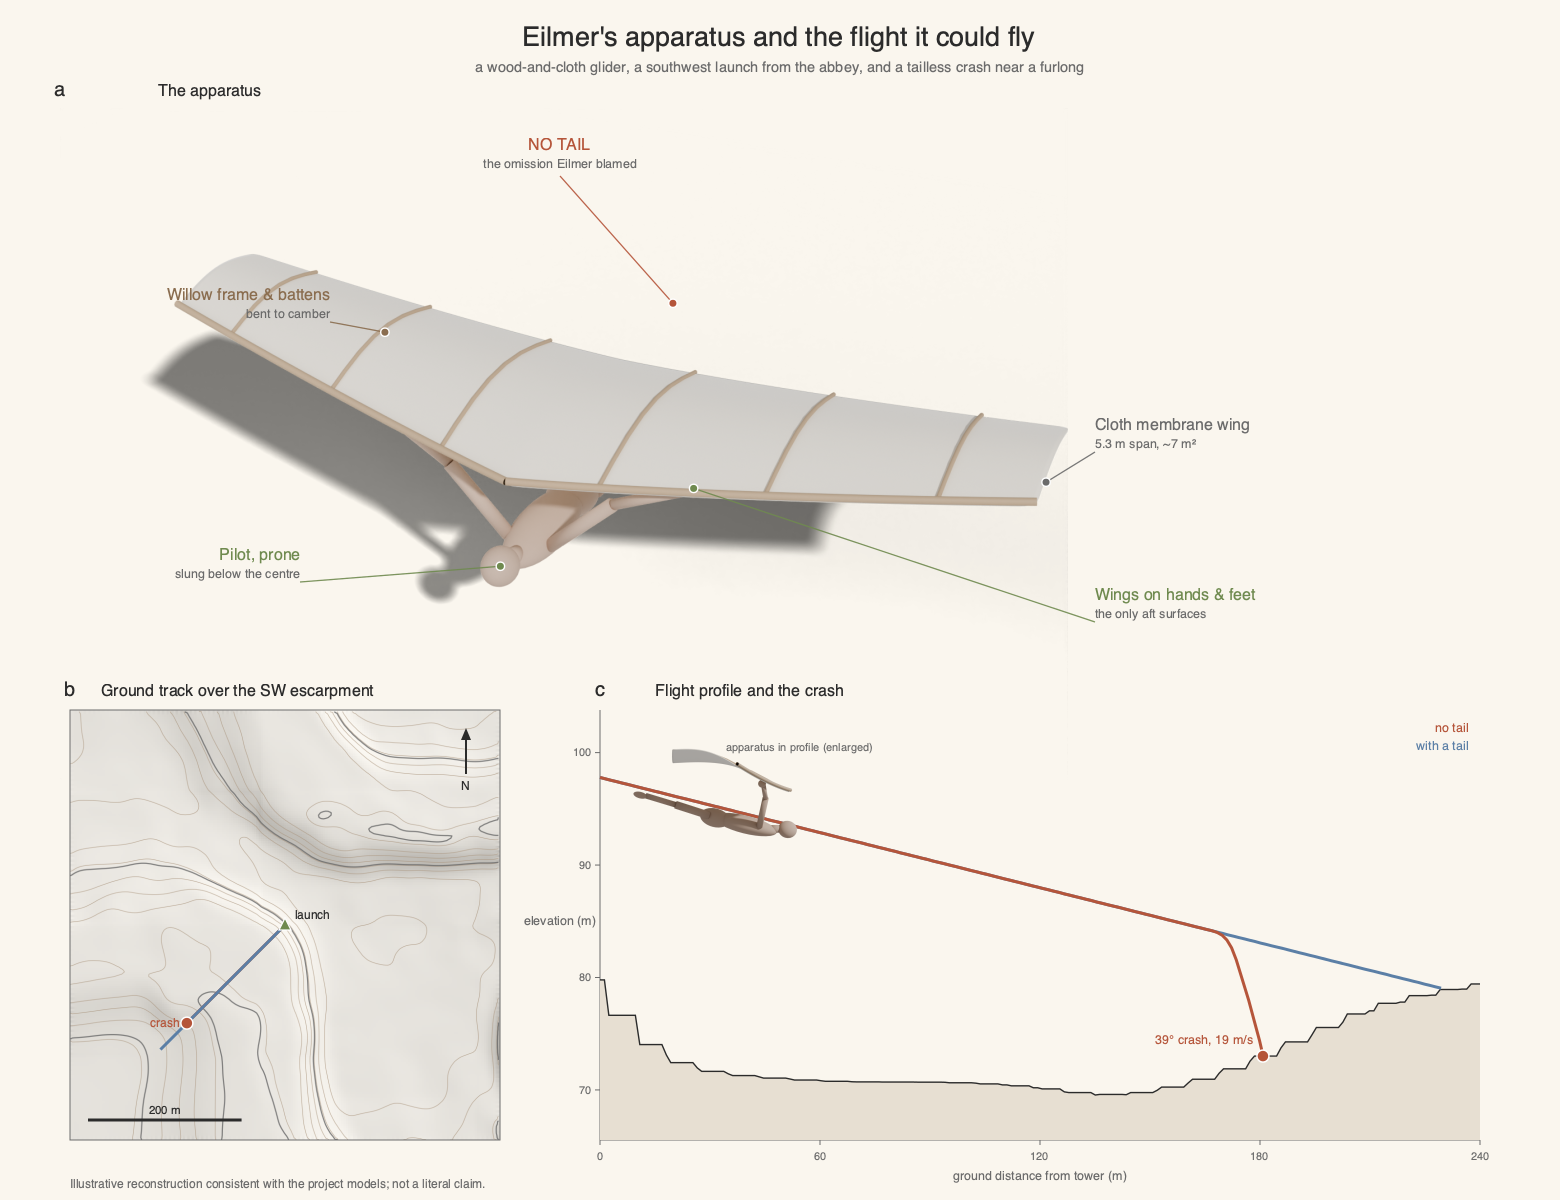
\includegraphics[width=\linewidth]{apparatus_flight.png}
  \caption{\textbf{Eilmer's apparatus and the flight it could fly.}
  \textbf{(a)} A to-scale reconstruction of the apparatus implied by the glide and
  stability models: a cambered cloth-membrane wing of about \SI{7}{\meter\squared}
  and \SI{5.3}{\meter} span (aspect ratio 4) on a willow frame, the pilot prone with
  wings fixed to the hands and feet and, as William of Malmesbury records, no tail.
  \textbf{(b)} Launch geometry on the abbey promontory, with the southwest ground
  track of the glide over a contour map of the escarpment, from the tower to an
  impact about a furlong away.
  \textbf{(c)} The flight in profile, apparatus enlarged for clarity: a
  wind-and-slope-assisted glide with a tail (blue) against the tailless case (red),
  which loses pitch control and strikes the ground at about \ang{39} and
  \SI{19}{\meter\per\second}.
  The reconstruction is illustrative and consistent with the project models, not a
  literal depiction.}
  \label{fig:apparatus}
\end{figure}

We treat the flight as a constrained engineering problem and attack it with the
tools available in 2026: a digital terrain model of the abbey promontory, two
decades of reanalysis wind climatology, a first-order orographic lift model, a
glide and short-period pitch-stability analysis, a Monte Carlo over the unknown
apparatus geometry and launch day, and an impact-biomechanics model calibrated to
human long-bone fracture tolerances.
\Cref{fig:apparatus} summarises the reconstruction and the result.
The contribution is twofold: a calibrated verdict on a specific historical claim,
and a reproducible method for adjudicating pre-modern flight accounts from terrain,
climate, and first-principles flight dynamics rather than from anecdote.
Everything here rebuilds from raw data with a single command, and the apparatus we
infer is a consequence of the models, not an input to them.
